\subsection{Aplicaciones de IoT}

\textbf{Comunicación y monitoreo}

El IoT tiene una amplia gama de aplicaciones en diversos sectores como se muestra en la ilustración No. 1. En el ámbito de la salud, el IoT se utiliza para monitorear pacientes y proporcionar atención médica remota. En el transporte, el IoT permite la gestión de flotas de vehículos y el seguimiento en tiempo real de la ubicación de mercancías. En la agricultura, el IoT se aplica para el monitoreo y control de cultivos, optimizando el riego y la fertilización. Además, el IoT ha encontrado aplicaciones en ciudades inteligentes, hogares inteligentes, industria manufacturera, entre otros campos.

\begin{figure}[htb]
	\centering
	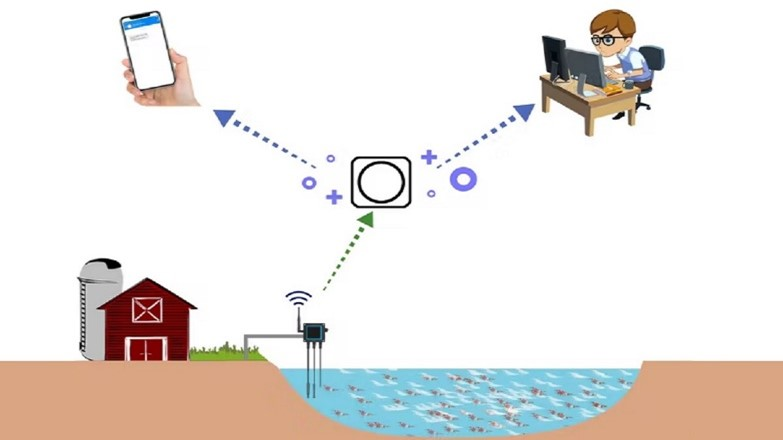
\includegraphics[scale  = 0.80]{Imagenes/iot.jpg}
	\caption{Sistema de monitoreo de acuicultura - Tecnologia Humanizada}{Fuente: Adaptado de~\cite{udin}}
\end{figure}

Sin embargo, la implementación exitosa de IoT en la recolección de residuos sólidos requiere de un enfoque integral que abarque aspectos técnicos, operativos y de privacidad de los datos. En la literatura científica existen algunos trabajos con propósitos similares que utilizan metodologías, arquitecturas y equipos diferentes, a continuación, se detallan.

Tarandeep Singh, en su trabajo denominado \textit{IOT based Smart Waste Management Framework (Singh)}, proporciona una solución para mejorar la gestión de residuos sólidos mediante la monitorización remota de los parámetros de los contenedores de basura y la optimización de las rutas de recolección. La metodología utiliza la tecnología X-bee y GSM para monitorear de forma remota los parámetros de los contenedores, como el llenado del contenedor, la temperatura, la humedad y el volumen de CO2 dentro del contenedor. Los datos recopilados se transmiten a una estación base que los envía a una estación de control para su análisis y optimización de rutas de recolección de basura. Las conclusiones del estudio sugieren que el uso de tecnología IoT en la gestión de residuos sólidos puede ser una solución efectiva y rentable para mejorar la eficiencia de la recolección de basura y reducir los costos operativos y las emisiones de gases de efecto invernadero.

Mientras tanto, Raúl Hernández y su equipo analizan la gestión y el proceso de recolección de residuos sólidos urbanos (RSU) en el municipio de Nezahualcóyotl, Estado de México, donde identifican las principales características de la gestión y recolección de RSU en el municipio y aplican la idea de la Ciudad Inteligente (CI) para mejorar el servicio de recolección de basura \cite{sinaluisa}.

La aplicación del Internet de las Cosas (IoT) en sistemas de clasificación de basura es una tendencia innovadora para mejorar la gestión de residuos. 

Sistemas de clasificación automática basados en cámaras y sensores ópticos conectados a la red IoT pueden identificar diferentes tipos de residuos (plásticos, metales, vidrio, etc.). Esto mejora la eficiencia del reciclaje al separar automáticamente los residuos según su tipo.

\begin{figure}[htb]
	\centering
	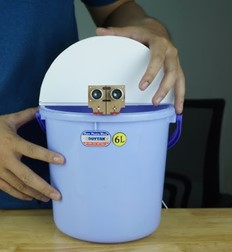
\includegraphics[scale  = 0.90]{Imagenes/iot_contenedor.jpg}
	\caption{IoT - contenedor de basura inteligente}{Fuente: Adaptado de~\cite{logic}}

\end{figure}

Las plataformas IoT permiten a los gestores de residuos monitorear remotamente el estado de los contenedores y otros equipos en tiempo real, lo que mejora la eficiencia operativa y reduce el tiempo de inactividad.